\chapter{LINE ATOMIC PARAMETERS}
% !TEX root = hazy2.tex

\section{Overview}

Many atomic physics quantities describe how matter and light interact.
This section goes over these quantities and how they are related to one
another.
The inter-relations between these quantities are described in most
spectroscopy texts, at about the same depth as is given below.  \citet{Hilborn1982} gives a far more formal description,
often tracing quantities back
to basic E\&M concepts.  Highly recommended.

\section{Spectroscopic notation}

A great deal of confusion exists over the difference between the
designation of a spectrum and an ion.  ``Atom~II'' denotes a spectrum, a
collection of photons, while ``Atom$^+$'' denotes a baryon,
the element ``Atom'' with a single electron removed.

Much of the notation in today's atomic physics was developed in the second
half of the 19th century.
Physicists noticed that the spectrum of a gas
would change dramatically when it was heated to high temperatures.
They
did not understand the reason why this happened,
the electron had not yet been discovered,
but they developed the
notation that ``Atom~I'' was the normal spectrum,
this spectrum changed
to ``Atom~II'' when the gas was heated,
and became the ``Atom~III'' spectrum if heated still further.
The ``Atom~II'' spectrum was often called the
``enhanced'' spectrum of Atom.
This is the reason why, in classical novae,
the appearance of broad absorption lines of singly ionized species
is called
the ``diffuse enhanced phase''.

The electron was discovered well after this notation had been developed.
By the early 20th century it was understood that the ``I'' spectrum was
produced by the atom, Atom$^0$.
At high temperatures the first ion, Atom$^+$,
formed and produced the ``Atom~II'' spectrum.

During the first half of the 20th century astrophysicists mainly studied
stellar absorption lines.
This led to the commonly-used notation that the
``Atom~II'' spectrum, for instance, measured Atom$^+$.
It is unambiguously true
that the equivalent width of an Atom~II absorption line is proportional
to the column density of Atom$^+$.
However there is an ambiguity in emission
lines.
The \la\ \hi\ line can be produced by impact excitation
of \hO\ or by recombination of \hplus.
In both cases the line is an \hi\ line, but \hi\ is
produced by either \hO\ or \hplus, depending on details.

To be unambiguously correct you should refer to Atom~I or Atom~II when
discussing the spectrum.
When discussing a column density or particle
density you should refer to the ion, as in Atom$^0$ or Atom$^+$.
It is not correct
to refer to the column density of \hi.
The \la\ \hi\  emission
line measures the column density of either \hO\ or \hplus,
depending on whether the line forms by impact excitation or recombination.
The notation is not ambiguous in absorption lines, which is probably why
we have such confusion today.
Be unambiguous and correct - use the right notation!

\section{Line absorption}

\subsection{Line optical depths}

The optical depth for a transition $u-l$,  where $u$ and $l$ are the upper
and lower levels, is given by
\begin{equation}
\label{eqn:OpticalDepthIncrement}
d{\tau _{l,u}} = {\alpha _\nu }\left( {{n_l} - {n_u}{g_l}/{g_u}}
\right)\;f(r)\;dr
\ [\mathrm{Napier}].
\end{equation}
Here $f (r)$ is the filling factor and $\alpha _\nu$ is the
atomic absorption cross section [cm$^2$].

The term in parenthesis is the population [cm$^{-3}$] of the lower level,
with a correction for stimulated emission.
This term is the only place where
stimulated emission enters in the radiative balance equations (\citealp{Elitzur1983}).

\subsection{Oscillator strengths}

The oscillator strength $f$ is a dimensionless number of order unity that
can be thought of as a correction factor to make the expression for a
classical oscillator agree with the quantum mechanical value.
Sections
below relate the oscillator strength to other line parameters such as the
absorption coefficient and the transition probability.
The absorption
($f_{abs}$,
called $f_{l,u}$ here) and emission ($f_{em}$, called $f_{u,l}$)
oscillator strengths are related~by
\begin{equation}
{g_l}{f_{l,u}} =  - {g_u}{f_{u,l}}% (2)
\end{equation}
where the $g$'s are the statistical weights.
This product is symmetric,
neglecting sign, and the code tries to use $gf$'s throughout.
The convention
is that emission lines have negative oscillator strength.

\subsection{Absorption cross section}

The absorption cross section [$\scm$] for a line is related to the
dimensionless absorption oscillator strength $f_{lu}$ or $f_{abs}$ by
\begin{equation}
\label{eqn:LineAbsorptionCrossSection}
\begin{array}{ccl}
 {\alpha _\nu(x) }& =& \frac{{{\pi ^{1/2}}q_e^2\lambda
\,{f_{l,u}}}}{{{m_e}c{u_{\rm Dop}}}}{\varphi _\nu }(x) \\
& =& 0.014974{f_{l,u}}\frac{{{\lambda_{\rm cm}}}}{{{u_{\rm Dop}}}}{\varphi _\nu
}(x) = 1.4974 \times {10^{ - 6}}{f_{l,u}}\lambda_{\mu\rm m}\frac{\varphi_\nu(x)}{u_{\rm Dop}} \\
 \end{array}
\quad [\mathrm{cm}^2]
\end{equation}
with the relative line displacement given by
\begin{equation}
\label{eqn:RelativelineDisplacement}
x \equiv \frac{{\nu  - {\nu _o}}}{{\Delta {\nu _{Dop}}}} ,
\end{equation}
${\varphi _\nu }\left( x \right)$
is the Voigt function, and $u_{\rm Dop}$ is the Doppler velocity width
(cm~s$^{-1}$), the
point where the line profile falls to 1/e of its peak.
With this definition
of the relative line displacement, the line profile due to thermal motions
alone is $\exp(-x^2)$.
The constant part of equation~\ref{eqn:LineAbsorptionCrossSection}
(i.e., everything except the rightmost term) is evaluated
in routine \cdRoutine{abscf}.

The Doppler width for thermal broadening of an atom with atomic mass A is
\begin{equation}
u_{Dop} = \left ( \frac{2kT}{m} \right )^{1/2} [\cmps ] = 
12.85 \left ( \frac{T}{10^4 A} \right )^{1/2} [\kmps ]
\end{equation}
(equation 9-35 of \cite{1970stat.book.....M}).

\section{The line profile function}

\subsection{Velocities in a thermal distribution}

The distribution function for a Maxwellian velocity distribution is
given by
\begin{equation}
\frac{{n\left( u \right)du}}{n} = \frac{1}{{{\pi ^{3/2}}}}\exp \left[
{ - {{{u^2}{m_A}} /
{2kT}}}
\right]{\left( {\frac{m}{{2kT}}}
\right)^{3/2}}4\pi {u^2}\,du\quad [\mathrm{cm~s}^{-1}]
\end{equation}
(\citealp{Novotny1973}; p 122).
There are three mean speeds in a thermal velocity
distribution.  The \cdTerm{most probable speed} is the peak
of the velocity
distribution, with a value
\begin{equation}
u_{mean}^2 = 2kT/{m_A}\quad[\mathrm{cm}^2 \; \mathrm{s}^{-2}].
\end{equation}
This is found by setting the derivative of the distribution function to
zero (\citealp{Novotny1973}, p 122).
The velocity distribution function can be
expressed in terms of the \cdTerm{mean speed} as
\begin{equation}
\frac{{n\left( u \right)du}}{n} = \frac{1}{{{\pi ^{3/2}}}}\exp \left[
{ - {{{u^2}} /{u_{mean}^2}}}\right]\frac{{4\pi
{u^2}}}{{u_{mean}^3}}\,du\quad [\mathrm{cm~s}^{-1}].
\end{equation}
The \cdTerm{average speed} is obtained by averaging over this function
and is given by
\begin{equation}
u_{average}^2 =8kT/\pi\, m_A\quad [\mathrm{cm}^2 \; \mathrm{s}^{-2}].% (8)
\end{equation}
The \cdTerm{thermal Doppler velocity width} is the
velocity averaged over the
projected line of sight, given by (\citealp{Novotny1973}; p 204)
\begin{equation}
u_{th}^2 = 2kT/{m_A}
\quad [\mathrm{cm}^2 \; \mathrm{s}^{-2}].
\end{equation}
This is the distance from line center where the line profile
falls to $e^{-1}$ of its central value.
So it turns out that the most probable speed is equal
to the Doppler velocity width.

The \cdTerm{velocity dispersion} $\sigma$ is
\begin{equation}
\sigma  = u/\sqrt 2
\quad [\mathrm{cm~s}^{-1}]% (10)
\end{equation}
and appears in the Gaussian profile function as
\begin{equation}
\varphi \left( {\delta u} \right) = \exp \left( { -
{\raise0.7ex\hbox{${\delta {u^2}}$} \!\mathord{\left/
 {\vphantom {{\delta {u^2}} {2{\sigma ^2}}}}\right.\kern-\nulldelimiterspace}
\!\lower0.7ex\hbox{${2{\sigma ^2}}$}}} \right).% (11)
\end{equation}

\subsection{Micro vs macro turbulence}

Micro-turbulence (hereafter, just turbulence) is due to any additional
motions that occur over scales that are smaller than a photon mean free
path.
Micro-turbulence changes the line transfer since the line opacity
is distributed over a broader range of velocities.
Macro-turbulence is
due to motion that occurs over such large scale lengths that they not change
the optical depth through the emitting region.
An example might be cloud
orbital motions.
The transfer within a cloud is not changed by its bulk
motion and so would be considered macro-turbulence.

\subsection{Line Widths}

If a non-thermal micro-turbulent component of motions is present then
equation \ref{eqn:LineAbsorptionCrossSection},
the total Doppler velocity width [cm~s$^{-1}$] including turbulence,
is given by
\begin{equation}
u_{tot}^2 = 2kT/{m_A} + u_{turb}^2
\quad[\mathrm{cm}^2 \; \mathrm{s}^{-2}]
\end{equation}
as determined by the local kinetic temperature $T$.
Within the code the
micro-turbulent velocity $u_{turb}$ is assumed to be zero
unless it is reset
with the \cdCommand{turbulence} command.\footnote{Note that the
\cdCommand{turbulence} command accepts $u_{turb}$ in $\kmps$ but converts
it into $\cmps$, the units used throughout the code.}

In \cdRoutine{GetDopplerWidth} the Doppler velocity width is evaluated as
\begin{equation}
{u_{Dop}} = \sqrt {2kT/{m_A} + u_{turb}^2}  = \sqrt {1.651 \times
{{10}^8}\,T/{m_{AMU}} + u_{turb}^2}
\quad  [\cmps].
\end{equation}
The atomic weight is in atomic mass units.

The Doppler velocity width is related to the half width at half maximum
by (\citealp{Novotny1973}, eqns 5-18; p 205)
\begin{equation}
\Delta {u_{1/2}} = {\left( {\ln 2} \right)^{1/2}}{u_{Dop}} =
0.832555\,{u_{Dop}}
\quad  [\mathrm{cm~s}^{-1}]
\end{equation}
and the FWHM is given by
\begin{equation}
\Delta {u_{FWHM}} = 2{\left( {\ln 2} \right)^{1/2}}{u_{Dop}}
\quad [\mathrm{cm~s}^{-1}].
\end{equation}

\subsection{The Doppler $b$ parameter}

Much of the literature refers to the Doppler $b$ parameter.
This is the
Doppler velocity width or velocity dispersion with turbulence included,
and is given by
\begin{equation}
{b^2} = u_{Dop}^2 = 2kT/{m_A} + u_{turb}^2
\quad [\mathrm{cm}^2 \mathrm{s}^{-2}].
\end{equation}
With these definitions
\begin{equation}
b = {u_{Dop}} = \Delta {u_{FWHM}}/\left[ {2{{\left( {\ln 2} \right)}^{1/2}}}
\right]
\quad  [\mathrm{cm~s}^{-1}].
\end{equation}

\subsection{Voigt function}

By combining equations~\ref{eqn:OpticalDepthIncrement} and \ref{eqn:LineAbsorptionCrossSection}
we can define the optical depth a relative displacement $x$ away from line center
as:
\begin{equation}
\label{eqn:LineOpticalDepth}
\tau_\nu(x) = \int_{R_{\rm in}}^{R_{\rm out}} \frac{{{\pi ^{1/2}}q_e^2\lambda
\,{f_{l,u}}}}{{{m_e}c{u_{\rm Dop}}}}\;{\varphi _\nu }(x)
\left({{n_l} - {n_u}{g_l}/{g_u}}\right)\;f(r)\;dr.
\end{equation}
Using this equation, the line center optical depth $\tau_0$ can be defined as
$\tau_0 \equiv \tau_\nu(0)$.
The relative displacement $x$ is given by
equation \ref{eqn:RelativelineDisplacement} above.
In our formalism, the Voigt function
is normalized such that the integral is $\sqrt\pi$.
A schematic approximation for the Voigt function is given by equation 9-61 of \citet{Mihalas1978}
\begin{equation}
\label{eqn:VoigtFunctionApproximation}
{\varphi _\nu }(x) \approx \exp ( - {x^2}) + a/({\pi ^{1/2}}{x^2}) .
\end{equation}
Here $a$ is the damping constant. This expression cannot be used in real
calculations as it goes to infinity for $x=0$, but it does convey the general
behavior of the Voigt function where for small $x$ it looks like a Gaussian
function while for large x it resembles a Lorentzian profile. In \Cloudy\ we
use an enhanced version of the \cdRoutine{humlik} algorithm \citep{Wells1999}
to calculate the Voigt function to a relative precision of at least
$2.5\times10^{-3}$ for all values of $a$ and $x$. For most values of $a$, the
relative accuracy will be better than $10^{-4}$ though.
The value at line center is given by:
\begin{equation}
\label{eqn:VoigtFunctionCenter}
{\varphi _\nu }(0) = 1 - \frac{2 a}{\sqrt\pi} + a^2 + O(a^3)\ (a \rightarrow 0).
\end{equation}
The line center optical depth thus depends on $a$, or more generally on the
shape of the line profile, while the mean optical depth does not.

\subsection{Mean vs. line center optical depths}

\Cloudy\ internally works with line center optical depths throughout (see, for
example, \citealp{Mihalas1978}). However, mean optical depths are reported in
the final printout. Since \Cloudy\ treats line overlap and also integrates the
line optical depth through a medium where the Doppler width will generally be
varying, it is not straightforward to convert the line center optical depths
used internally to a mean optical depth. To avoid these difficulties, we
report a mean optical depth that is exactly a factor $\sqrt\pi$ times
\emph{larger} than the line center optical depth. This assumes that the Voigt
function at line center is ${\varphi _\nu }(0) \approx 1$. This approximation
is OK when the damping parameter $a$ is small, $a\ll1$ (see
equation~\ref{eqn:VoigtFunctionCenter}), which is generally the case in the
IR, optical, and UV wavelength range. However, this approximation breaks down
in the X-ray regime where $a$ can be much larger.

\section{The Einstein coefficients}

The dimensionless oscillator strength $gf$ is related to the transition
probability $A_{ul}$ [s$^{-1}$]~by
\begin{equation}
{g_l}{f_{l,u}} = {g_u}{f_{u,l}} = \frac{{{m_e}c\lambda _{cm}^2}}{{8{\pi
^2}q_e^2}}{g_u}{A_{u,l}} = 1.4992{g_u}{A_{u,l}}\lambda _{cm}^{\,2} = 1.4992
\times {10^{ - 8}}{g_u}{A_{u,l}}\lambda _{\micron}^{\,2}
\end{equation}
where $\lambda_{\micron}$ is the wavelength in microns and $\lambda_{cm}$ the wavelength in centimeters.
The absorption oscillator strength is related to the
transition probability by
\begin{equation}
\label{eqn:gfAulRelation}
{f_{l,u}} = \frac{{{m_e}c\lambda _{cm}^2}}{{8{\pi
^2}q_e^2}}\frac{{{g_u}}}{{{g_l}}}{A_{u,l}} = 1.4992 \times {10^{ -
8}}{A_{u,l}}\lambda _{\mu m}^{\,2}\frac{{{g_u}}}{{{g_l}}}
\end{equation}
or
\begin{equation}
{A_{u,l}} = \frac{{8{\pi ^2}q_e^2}}{{mc\lambda
_{cm}^2}}\frac{{{g_l}}}{{{g_u}}}{f_{abs}} = \frac{{{f_{l,u}}}}{{1.4992 \times
{{10}^{ - 8}}}}\lambda _{\mu m}^{ - \,2}\frac{{{g_l}}}{{{g_u}}}\quad
[\mathrm{s}^{-1}].
\end{equation}
Combining equations \ref{eqn:LineAbsorptionCrossSection}
and \ref{eqn:gfAulRelation} we obtain an expression relating the
transition probability and the absorption cross section;
\begin{equation}
\begin{array}{ccl}
 {\alpha _\nu }& =& \frac{{{\lambda ^3}{g_u}}}{{8\pi
{g_l}}}\frac{{{A_{u,l}}}}{{{\pi ^{1/2}}{u_{Dop}}}}{\varphi _\nu }\left(
x \right) \\
&=& \frac{{{\lambda ^3}{g_u}}}{{8\pi {g_l}}}\frac{{{A_{u,l}}}}{{{\pi
^{1/2}}{u_{Dop}}}}{\varphi _\nu }\left( x \right) \\
&=& 2.24484 \times {10^{ - 14}}{A_{u,l}}\lambda _{\mu
m}^{\,3}\frac{{{g_u}}}{{{g_l}}}\frac{{{\varphi _\nu }\left( x
\right)}}{{{u_{Dop}}}} \\
 \end{array}
\quad  [\mathrm{cm}^2].
\end{equation}
The coefficient for induced emission,
$B_{ul}$, is related to $A_{ul}$ by the phase
space factor $2h{\nu ^3}/{c^2}$;
\begin{equation}
{A_{u,l}} = \frac{{2h{\nu ^3}}}{{{c^2}}}{B_{ul}}
\quad [\mathrm{s}^{-1}]
\end{equation}
and the induced emission and absorption probabilities are related by
\begin{equation}
{g_l}{B_{l,u}} = {g_u}{B_{u,l}}
\end{equation}
The absorption cross section $\alpha _v$ is related to $B_{l,u}$ by
\begin{equation}
{\alpha _\nu }\, = \frac{{hc}}{{4{\pi
^{3/2}}}}\frac{{{B_{l,u}}}}{{{u_{Dop}}}}{\varphi _\nu }\left( x \right)
\quad [\mathrm{cm}^2].
\end{equation}
In these terms the optical depth increment
(equation \ref{eqn:OpticalDepthIncrement}) is given by
\begin{equation}
\begin{array}{ccl}
 d{\tau _{l,u}}& =& {\alpha _\nu }\left( {{n_l} - {n_u}{g_l}/{g_u}}
\right)f\left( r \right)\,\,dr \\
& =& \frac{{hc}}{{4{\pi ^{3/2}}}}\frac{{{B_{l,u}}}}{{{u_{Dop}}}}{\varphi
_\nu }\left( x \right)\left( {{n_l} - {n_u}{g_l}/{g_u}} \right)f\left( r
\right)\,dr \\
 \end{array}
 .
\end{equation}

\section{Continuum pumping}

\subsection{Photon occupation number}

The intensity of a radiation field can be thought of as two parts, the
available volume of phase space $2h{\nu ^3}/{c^2}$
and a dimensionless occupation number $\eta$ giving the fraction
of that space that is filled.
Occupation numbers can be larger than unity for
photons, which are Bose-Einstein particles.

For reference, the Planck function is given by
\begin{equation}
{B_\nu } = {I_\nu } = \frac{{{F_\nu }}}{\pi } = \frac{{2h{\nu
^3}}}{{{c^2}}}\frac{1}{{\exp \left( {h\nu /kT} \right) - 1}}
\quad  [\mathrm{erg~cm}^{-2}\;\mathrm{s}^{-1}\; \mathrm{sr}^{-1}\; \mathrm{Hz}^{-1}]% (28)
\end{equation}
where $F_\nu$ is the single-hemisphere emittance from an opaque surface.
The photon occupation number of a blackbody is then
\begin{equation}
\label{eqn:PhotonOccupationNumber}
{\eta _\nu } = \frac{1}{{\exp \left( {h\nu /kT} \right) - 1}}
\end{equation}
The dimensionless occupation number for any continuum with a mean intensity
$J_\nu$ (erg~cm$^{-2}$~s$^{-1}$~Hz$^{-1}$ sr$^{-1}$) at a frequency $\nu$ is defined as
\begin{equation}
{\eta _\nu } \equiv {J_\nu }/\left( {2h{\nu ^3}/{c^2}} \right) \equiv
{\left[ {\exp \left( {h\nu /k{T_{ex}}} \right) - 1} \right]^{ - 1}}
.
\end{equation}
Here $T_{ex}$ is the excitation temperature of the continuum at the frequency.

\subsection{Pumping rates}

Continuum fluorescence is treated as in \citet{Ferland1988} and \citet{Ferland1992}.
The rate of induced radiative excitation by continuum photons
(continuum pumping) is given by
\begin{equation}
{r_{l,u}} = {n_l}{B_{l,u}}{J_{l,u}} =
{n_l}{A_{u,l}}\frac{{{J_{l,u}}}}{{2h{\nu ^3}/{c^2}}}\frac{{{g_u}}}{{{g_l}}}
= {n_l}{A_{u,l}}{\eta _\nu }\frac{{{g_u}}}{{{g_l}}}
\quad [\mathrm{cm}^{-3}\;\mathrm{s}^{-1}]
\end{equation}
where $\eta_\nu$ is the dimensionless continuum occupation number
at the line energy.
The rate of induced radiative de-excitation is related by
detailed balance and is given by
\begin{equation}
{r_{u,l}} = {r_{l,u}}\frac{{{g_l}}}{{{g_u}}}
\quad [\mathrm{cm}^{-3} \;\mathrm{s}^{-1}].
\end{equation}
The occupation number has the advantage that the Einstein $B$'s
do not enter any rate equations.
All radiative rates can be expressed in terms of an
$A$ and $\nu$.

\subsection{Optical depth effects}

The line becomes self-shielding when the optical depth is greater than
unity.
The line optical depth between the current position and the
illuminated face of the slab is used to evaluate the inward-looking escape
probability, the probability that a line photon will travel this distance
in a single scattering.
Line optical depths do not directly affect $\eta_c$,
only continuous opacities do.
The final form of the continuum pumping rate is
\begin{equation}
{r_{l,u}} = {n_l}{A_{u,l}}{\eta _\nu }\frac{{{g_u}}}{{{g_l}}}{\gamma
_{l,u}}\left( \tau  \right)
\quad [\mathrm{cm}^{-3} \;\mathrm{s}^{-1}]
\end{equation}
where $\gamma_{l,u}$ is the probability that continuum photons
penetrate an optical
depth $\tau_o$ and are then absorbed by an atom:
\begin{equation}
{\gamma _{l,u}} = \int_0^\infty  {{\varphi _\nu }\;\exp \left( { - {\tau
_o}{\varphi _\nu }} \right)\,d\nu } /\int_0^\infty  {{\varphi _\nu }\;d\nu
} .
\end{equation}
where $\varphi_\nu$ is the Voigt function.
Figure \ref{fig:pump_probability},
taken from \citet{Ferland1992}, shows
$\gamma_{l,u}$ for a wide variety of values of the damping constant $a$.

\begin{figure}
\centering
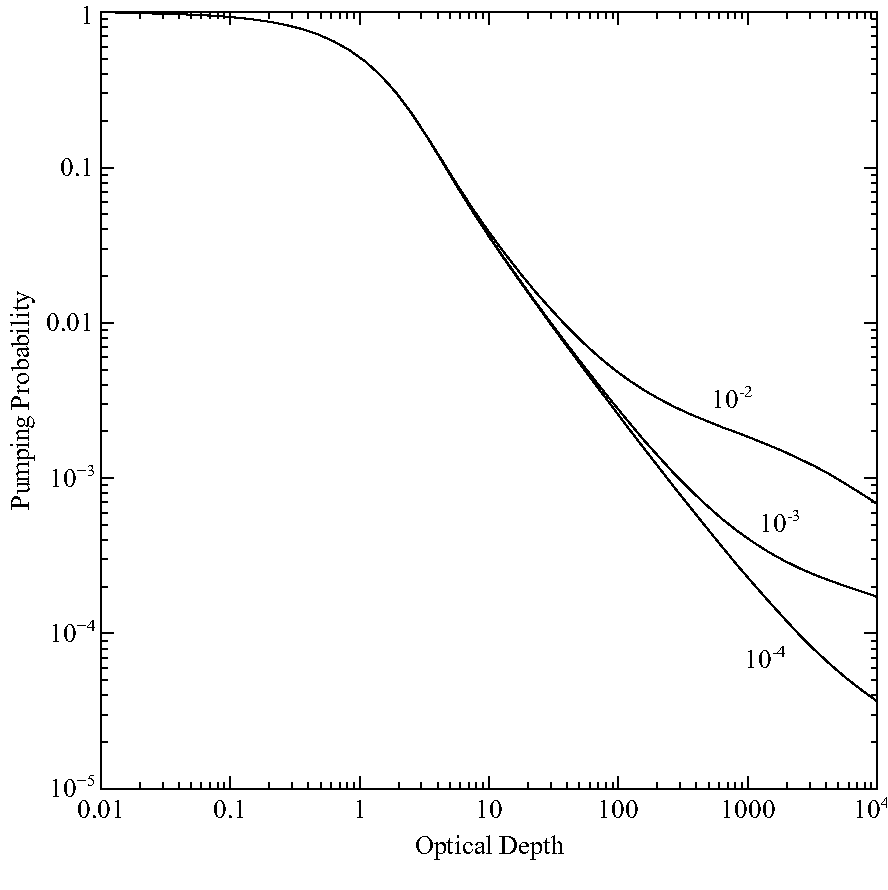
\includegraphics[scale=0.8]{pump_probability}
\caption[Fluorescent pumping probability]{\label{fig:pump_probability}This figure
shows the probability that a photon will penetrate
to the line center optical depth shown on the x-axis, and then be absorbed
by the line.  The curves are for various values of the damping constant
a (the ratio of damping width to Doppler width), as indicated on the
figure.}
\end{figure}

The code works in terms of the flux of photons per energy mesh point.
The transmitted continuum has a flux of photons $\varphi_\nu$
(photons cm$^{-2}$ s$^{-1}$ Ryd$^{-1}$).
The photon occupation number of the attenuated continuum is given by equation \ref{eqn:PhotonOccupationNumber} above, here written as
\begin{equation}
{\eta _\nu } = {\varphi _\nu }\;\frac{{{c^2}}}{{8\pi \;\nu _1^3\;\nu
_{Ryd}^2}}
\end{equation}
where $\nu_{Ryd}$ is the frequency in Rydbergs,
$\nu_1$ is the frequency of 1 Rydberg,
and the other symbols have their usual meaning.
Continuum pumping is
included among the general line excitation processes for all lines
considered by the code.

\section{Kirchhoff's Law}

Kirchhoff's law is the statement that, in thermodynamic equilibrium,
the energy emitted is equal to the energy absorbed.  If the emission and
absorption coefficients are $j_{\nu}$ and $\kappa_{\nu}$ then
\begin{equation}
j_{\nu} = \kappa_{\nu} B_{\nu}(T)
\end{equation}
where $B_{\nu}(T)$ is Planck's function.

\section{The line source function and mean intensity}

The source function for a line is defined as
\begin{equation}
{S_l}\left( {{T_{exc}}} \right) \equiv {B_l}\left( {{T_{exc}}} \right)
\equiv \frac{{{j_l}}}{{{\kappa _l}}} =
\frac{{{A_{u,l}}{n_u}}}{{{B_{l,u}}\left( {{n_l} - {n_u}{g_l}/{g_u}}
\right)}}
\quad
  [\mathrm{erg~Hz}^{-1}\; \mathrm{sr}^{-1}\; \mathrm{s}^{-1}].
\end{equation}
where $T_{exc}$ is the line excitation temperature
\begin{equation}
\frac{{{n_u}/{g_u}}}{{{n_l}/{g_l}}} = \exp \left[ { - h\nu /k{T_{exc}}}
\right]
\end{equation}
$B_l(T_{exc})$ is the Planck function at the line excitation
temperature and the
line emission and absorption coefficients $jl$ and $kl$
enter through Kirchhoff's law.
Combining with the definitions of the Einstein relations we find the
relation
\begin{equation}
{S_l}\left( {{T_{exc}}} \right) = \frac{{2h{\nu
^3}}}{{{c^2}}}\frac{{{n_u}/{g_u}}}{{\left( {{n_l}/{g_l} - {n_u}/{g_u}}
\right)}}
\quad  [\mathrm{erg~Hz}^{-1}\; \mathrm{sr}^{-1}\; \mathrm{s}^{-1}].
\end{equation}
The radiation field within the line is given by the mean intensity
$\bar J$.
$\bar J$  and $S_l$ are related by the net radiative bracket,
which we approximate as
the escape probability $P_{esc}$:
\begin{equation}
{P_{esc}} \equiv 1 - \bar J/{S_l}. %(40)
\end{equation}
The mean intensity is then give by
\begin{equation}
\bar J = {S_l}\left( {1 - {P_{esc}}} \right) .% (41)
\end{equation}
and the line center photon occupation number is
\begin{equation}
{\eta _l} = \frac{{{n_u}/{g_u}}}{{\left( {{n_l}/{g_l} - {n_u}/{g_u}}
\right)}}\left( {1 - {P_{esc}}} \right).
\end{equation}

\section{Level populations in radiative equilibrium limit}

For a two-level system where collisions can be neglected, in the optically
thin limit, the balance equation relating the populations of a two-level
system is given by
\begin{equation}
\frac{{d{n_u}}}{{dt}} = {n_l}{B_{lu}}J - {n_u}\left( {{A_{ul}} + {B_{ul}}J}
\right)
\quad  [\mathrm{cm}^{-3} \;\mathrm{s}^{-1}].
\end{equation}
In the time-steady limit, where the time derivative is zero, the balance
can be rewritten in terms of the transition probabilities as
\begin{equation}
{n_u}\left( {{A_{ul}} + {A_{ul}}\eta } \right) = {n_u}{A_{ul}}\left( {1
+ \eta } \right) = {n_l}{A_{ul}}\eta \frac{{{g_u}}}{{{g_l}}}
\quad  [\mathrm{cm}^{-3} \;\mathrm{s}^{-1}].
\end{equation}
In the limit where $\eta$ is small every photoexcitation is followed by
spontaneous decay, while in the limit where $\eta$ is large the level populations
are given by the ratio of statistical weights, i.e., $T_{exc}$ is infinite.



